\begin{appendices}
\crefalias{chapter}{appsec}
\chapter{Heat Equation Derivation}
\label{app:heatderive}

To derive the heat equation we consider the conversation of energy in a volume R, with a flux out, $\phi(x,y,z,t)$, and unit outer normal $\mathbf{\hat{n}}$. We need just the normal component of $\phi$ 
: $\phi \cdot \mathbf{\hat{n}}$.
\medskip

The rate of change of heat inside the volume R is equal to the heat generated inside the volume R plus the heat flowing in/out of the boundary surface:

\begin{equation}
\parbox{70pt}{Rate of change of heat energy}\ =\ \parbox{60pt}{Rate of heat generation in R} +\ \parbox{105pt}{Rate of heat energy flowing through boundary surface}
\label{eqn:word}
\end{equation}

\medskip
The total heat energy is:

\begin{equation}
e(x,y,z,t)=c(x,y,z)\cdot \rho(x,y,z)\cdot T(x,y,z,t)
\end{equation} 

and therefore the rate of change of heat energy is

\begin{equation}
\frac{d}{dt} \iiint\limits_{R} e\ dV= \frac{d}{dt}\iiint\limits_{R} c\rho T\ dV
\label{eqn:rotenergy}
\end{equation}

We denote the heat generated inside the volume R as $Q(x,y,z,t)$:

\begin{equation}
\iiint\limits_{R} Q\ dV
\label{eqn:rotheatgen}
\end{equation}

and the rate of heat energy flowing through the boundary surface is:

\begin{equation}
-\iint \limits_{\partial R} \phi\cdot \mathbf{\hat{n}}\ dS\footnote[3]{This is negative as outward flow $\phi$ is positive, but the flow would result in a reduction of energy.}
\label{eqn:rotheatloss}
\end{equation}

Substituting \cref{eqn:rotenergy,eqn:rotheatgen,eqn:rotheatloss} into \cref{eqn:word}, yields:

\begin{equation}
\frac{\partial}{\partial t} \iiint\limits_{R} c\rho T\ dV = -\iiint \limits_{R} \phi\cdot \mathbf{\hat{n}}\ dV +  \iiint\limits_{R} Q\ dV
\end{equation}

Using the divergence theorem, and simplifying gives: 

%\begin{equation}
%\iint \limits_{\partial R} \phi\cdot \mathbf{\hat{n}}\ dS = \iiint \limits_{R} \nabla\cdot \phi\ dV
%\end{equation}

\begin{equation}
\frac{\partial}{\partial t} \iiint\limits_{R} c\rho T\ dV = -\iiint \limits_{R} \nabla\cdot \phi\ dV +  \iiint\limits_{R} Q\ dV
\end{equation}

\begin{equation}
\iiint\limits_{R} \left[ c\rho \frac{\partial}{\partial t} T + \nabla\cdot \phi - Q\right] dV = 0
\end{equation}

Which holds for an arbitrary R, thus:

\begin{equation}
c\rho\frac{\partial}{\partial t}T = - \nabla \cdot \phi + Q
\label{eqn:heatpreq}
\end{equation}



Using Fourier's law of heat conduction, which states that the local heat flux density, $\phi$, is proportional to the negative local temperature gradient. The proportionality constant being equal to the thermal conductivity, $\kappa$:

\begin{equation}
\phi(x,y,z,t)=\kappa(x,y,z)\nabla T(x,y,z,t)
\label{eqn:fourier}
\end{equation}

Substituting \cref{eqn:fourier} into \cref{eqn:heatpreq} yields the heat equation:

\begin{equation}
c\rho\frac{\partial}{\partial t}T = \nabla\cdot (\kappa\nabla T) + Q
\end{equation}

Which can be simplified into the homogeneous medium heat equation with the following assumptions: Q=0 and $\kappa,\ \rho,\ and\ c$ are constant, and $\alpha=\tfrac{\kappa}{c\rho}$

\begin{equation}
\frac{\partial T}{\partial t} = \alpha \nabla^2 T
\end{equation}

%**************************************************************************************
\crefalias{chapter}{appsec}
\chapter{Fresnel Reflections}
\label{app:fresnelappend}

In order to be able to accurately model the paths that light take in a medium where the refractive indices varies, Fresnel reflections and refractions must be modelled.
To model these reflections and refractions in a simulation we calculate the Fresnel coefficients.
\Cref{eqn:fres1,eqn:fres2,eqn:frestot} shows the equations for calculating these for $s$ and $p$ polarised light, and unpolarised light (\cref{eqn:frestot}).


\begin{align}
R_s&=\left|\frac{n_1 \cos\theta_i-n_2\cos\theta_t}{n_1\cos\theta_i+n_2\cos\theta_t}\right|^2\label{eqn:fres1}\\
R_p&=\left|\frac{n_1 \cos\theta_t-n_2\cos\theta_i}{n_1\cos\theta_t+n_2\cos\theta_i}\right|^2\label{eqn:fres2}\\
R_{eff}&=\tfrac{1}{2}\left(R_s+R_p\right)\label{eqn:frestot}
\end{align}

\noindent Where: 

\indent $\theta_i$ and $\theta_t$ are the angle of incidence and angle of transmission respectively,

\indent see~\cref{eqn:sincos1,eqn:sincos2} and~\cref{fig:reflcfig,fig:transfig};

\indent $n_1$ and $n_2$ are the refractive indices of the current medium and the transmission medium [-];

\indent $R_s$ and $R_p$ are the reflectance coefficients for $s$ and $p$ polarised light respectively [-];

\indent finally, $R_{eff}$ is the effective reflective coefficient for unpolarised light [-].

\medskip

\begin{align}
\sin\theta_t&=\frac{n_1}{n_2}\sin\theta_i\label{eqn:sincos1}\\
\cos\theta_t&=\sqrt{1. - {\sin\theta_t}^2}\label{eqn:sincos2}
\end{align}

$R_{eff}$ gives a probability of reflection or refraction for a ray of light with an angle of incidence $\theta_i$.


To calculate the angles of reflection and refraction, a vector form of Snell's law is used.
Using the geometry illustrated in~\cref{fig:reflcfig} one can see that:

\begin{align}
I &= A+B\label{eqn:Ione}\\
R &= A-B\label{eqn:Rone}
\end{align}

\begin{equation}
B=\cos(\theta)\cdot N
\label{eqn:breflc}
\end{equation}

\begin{figure}[!htpb]
    \centering
    \includegraphics[width=0.35\textwidth]{reflc.pdf}
    \caption{Geometry for reflection of light at a refractive change boundary. I is incident light, R is the reflected light, and N is a normal to the surface. Here, $\theta$ is the angle of incidence which is equal to the angle of reflection.}
    \label{fig:reflcfig}
\end{figure}

Therefore, substituting~\cref{eqn:breflc} into~\cref{eqn:Ione,eqn:Rone} and rearranging yields:

\begin{align}
I&=A+\cos\left(\theta\right)\cdot N\\
R&=A-\cos\left(\theta\right)\cdot N
\end{align}
\begin{equation}
\therefore R=I-2(N\cdot I) N\label{eqn:reflcfin}
\end{equation}

Where $R$ gives the vector for a ray of light that has undergone reflection.
Next we treat the transmission case.
\Cref{fig:transfig} gives the geometry for the situation, where the circle is a unit circle.

\begin{figure}[!htpb]
    \centering
    \includegraphics[width=0.35\textwidth]{trans.pdf}
    \caption{Geometry of light refraction and reflections.}
    \label{fig:transfig}
\end{figure}

Again, one can deduce the following using trigonometry and~\cref{fig:transfig}:

\begin{align}
T&=A+B\label{eqn:Tone}\\
A&=\sin\left(\theta_2\right) M\label{eqn:Aone}\\
B&=\cos\left(\theta_2\right)(-N)\label{eqn:Btwo}\\
C&=\cos\left(\theta_1\right)N\label{eqn:Cone}\\
M&=\frac{I+C}{\sin\left(\theta_1\right)}\label{eqn:Mone}
\end{align}

Substituting~\cref{eqn:Aone,eqn:Btwo,eqn:Cone,eqn:Mone} into~\cref{eqn:Tone} and rearranging yields:

\begin{align}
T&=A+B\\
&=M\sin\theta_2-N\cos\theta_2\\
&=\frac{I+C}{\sin\theta_1}\sin\theta_2-N\cos\theta_2\\
&=\frac{(I+\cos\theta_1 N)\sin\theta_2}{\sin\theta_1}-N\cos\theta_2
\end{align}

\begin{equation}
\frac{\sin\theta_1}{\sin\theta_2}=\frac{\eta_1}{\eta_2}
\end{equation}

\begin{align}
\therefore T&=\frac{\eta_1}{\eta_2}\left(I+\cos\theta_1 N\right)-N\cos\theta_2\label{eqn:Tpenult}\\
T&=\eta+\left(\eta c_1-c_2\right)N\label{eqn:transfin}
\end{align}

Where~\cref{eqn:Tpenult} can be simplified by defining the following expressions:

\begin{align}
c_1 &= N \cdot I\label{eqn:c1}\\
c_2 &= \sqrt{1. - \eta^2 (1. - c_1^2)}\label{eqn:c2}\\
\eta&=\frac{\eta_1}{\eta_2}
\end{align}


To apply~\cref{eqn:reflcfin,eqn:transfin} to our voxel model, the algorithm checks if there is a change in refractive index whenever a photon packet moves into a new voxel.
If there is a change of refractive index the packet is placed on the surface of the voxel, and the algorithm calculates the surface normal of the voxel the light has hit and uses the above equations to calculate $R_{eff}$.
With $R_{eff}$ calculated a random number, $\xi$, is drawn.
If $\xi$ is less than $R_{eff}$ then the photon packet is reflected, else then the packet is refracted into the new voxel.
The new direction vectors are set according to~\cref{eqn:transfin,eqn:reflcfin} and the packet is propagated as normal.

%**************************************************************************************************************************************************************************************************************
\crefalias{chapter}{appsec}
\chapter{Detected Light Fluence Tracking Method}
\label{app:lightdect}

Most the fluence graphs presented in this thesis shows the fluence of the incident light throughout the simulated medium.
However, there are problems where tracking the fluence of the detected light maybe useful, though this quantity is not straight forward to track.
The current method of tracking fluence, is to add pathlengths, calculated as the packet moves from voxel to voxel to a 3D array. 
This method obviously cannot determine which packet will be detected before the packet is detected, therefore a new method must be devised.
This new method tracks the coordinates, direction vectors, random optical distance and fluorescent source of the packet using a stack.
A stack is a commonly used abstract data structure, and is a collection of elements.
In this case the elements are the coordinates, direction vectors, optical distance and fluorescent source.
A stack has two main operations, pop and push.
The push operation adds a new element to the collection, and the pop operation removes the most recently added element from the collection.
This is known as last in first out (LIFO).
\Cref{fig:stack} shows these two operations in action.

\begin{figure}[!htpb]
	\centering
	\includegraphics[width=0.35\textwidth]{stack.pdf}
	\caption{Example of the push and pop operation on a stack. The first operation add the integer 2 to the stack. The second operation push 7 to the stack. The last operation pops the 7 from the stack.}
	\label{fig:stack}
\end{figure}

The progress of each packet is pushed onto the stack, as it is propagated through the simulated medium. 
As mentioned above the packets coordinates, direction vectors, optical depth, and fluorescent source are the quantities pushed to the stack.
These quantities are pushed to stack every time an interaction event occurs.
When a packet is terminated, either via absorption or it leaving the medium, the packets details are removed from the stack.
This occurs unless the packet is detected.
If the packet is detected then the information remains on the stack.
This whole process repeats until all the packets have been run.
Once all the packets have been run, the packets are ``replayed''.
This is achieved by popping the information off the stack and passed to the inttau2 routine.
The packet is the propagated again, this time recording the fluence as done in most of the chapters in this thesis.

\end{appendices}
